\documentclass[11pt,a4paper]{article}
\usepackage[T1]{fontenc}
\usepackage[utf8]{inputenc}
\usepackage{mathpazo}
\usepackage{courier}
\usepackage{microtype}
\usepackage[margin=2.5cm]{geometry}
\usepackage{amsmath,amssymb,bm}
\usepackage{siunitx}
\sisetup{detect-all,per-mode=symbol,group-separator={\,},range-phrase={--}}
\usepackage{booktabs,array,tabularx,multirow,longtable}
\usepackage{graphicx}
\usepackage[labelfont=bf,font=small,labelsep=period]{caption}
\usepackage{float}
\usepackage{enumitem}
\setlist{nosep,leftmargin=1.4em}
\setlength{\emergencystretch}{3em}
\usepackage[authoryear,round]{natbib}
\setlength{\bibsep}{2pt}
\usepackage[colorlinks=true,linkcolor=blue!50!black,citecolor=blue!50!black,urlcolor=blue!50!black]{hyperref}
\usepackage{xcolor}

\newcommand{\code}[1]{\texttt{\detokenize{#1}}}
\newcommand{\CdA}{C_{\!d}A}
\newcommand{\dd}{\mathrm{d}}
\newcommand{\ts}{\hspace{0.15em}}
\DeclareMathOperator{\clip}{clip}
\DeclareMathOperator{\Var}{Var}
\DeclareMathOperator{\sgn}{sgn}

\title{\textbf{Physical Models of BikeToolsAnalyzer}\\[0.3em]
\large Cycling power balance and aerodynamic-drag (\(\CdA\)) estimation,\\
and a two-node model of core and skin temperature}
\author{Technical documentation\\[0.2em]\small\texttt{src/physics/aerodyn.py} and \texttt{src/physics/thermal.py}}
\date{29 October 2026}

\begin{document}
\maketitle

\begin{abstract}
\noindent
This report documents, derives and critically assesses the two physical models used by BikeToolsAnalyzer to interpret a recorded ride: (i) the \emph{road-cycling power balance}, which closes the balance between measured crank power and the sum of aerodynamic, rolling, gravitational and inertial power, and from which the effective drag area \(\CdA\) is estimated by least squares; and (ii) a lumped \emph{two-node thermoregulation model} (core and skin) that predicts core temperature from power, ambient temperature, humidity, air speed and clothing. For each model we state the governing equations, relate every term to the code, give the provenance of each constant, and quantify the behaviour of the implementation with controlled numerical experiments (Monte-Carlo recovery of a known \(\CdA\), first-order error propagation, step-size convergence, energy-conservation checks and parameter sensitivity). The audit identified and corrected several defects, which are listed in a findings register together with the limitations that remain. The main conclusions are: the least-squares \(\CdA\) estimator is unbiased where the per-sample-ratio estimator is biased by up to \SI{10}{\percent}, but its accuracy is limited by \emph{systematic} errors (grade, wind, rolling resistance) of the order \(0.01\)--\(0.04\ \si{m^2}\) rather than by random noise, and descents steeper than \SI{5}{\percent} are excluded because unmeasured braking there would otherwise be booked as drag (\(+15\%\) in a test ride). The thermal model is physically consistent and energy-conserving but \emph{uncalibrated}, with a strong dependence on the assumed gross efficiency (its exercise set point is driven by the rider's FTP), so it should be used for relative comparisons rather than as an absolute predictor of core temperature.
\end{abstract}

\tableofcontents
\newpage

%=====================================================================
\section{Scope and conventions}
%=====================================================================
The software reads a ride as a time series sampled at (nominally) \SI{1}{Hz}: ground speed \(v\), power \(P\), grade, altitude, heading (bearing), and --- from a weather service \citep{openmeteo} --- temperature, relative humidity, wind speed at \SI{10}{m} and the direction \emph{from which} the wind blows. Symbols are summarised in Table~\ref{tab:symbols}. Throughout, SI units are used; temperatures are in \si{\degreeCelsius}, and ``grade'' is the slope \(s=\tan\theta\) (a grade of \SI{5}{\percent} is \(s=0.05\)).

\begin{table}[H]
\centering\small
\begin{tabular}{@{}l>{\raggedright\arraybackslash}p{5.6cm}l>{\raggedright\arraybackslash}p{4.2cm}@{}}
\toprule
Symbol & Meaning & Unit & Code name \\
\midrule
\(P\) & power measured at the crank/pedals & W & \code{power} \\
\(\lambda\) & drivetrain loss fraction & --- & \code{DRIVETRAIN_LOSS} \\
\(m\) & total mass (rider + bike) & kg & \code{rider_mass}, \code{BIKE_MASS_KG} \\
\(v\) & ground speed (smoothed) & \si{m/s} & \code{speed} \\
\(v_a\) & air speed relative to rider, \emph{along} the road & \si{m/s} & \code{_air_speed} \\
\(\CdA\) & drag area (drag coefficient \(\times\) frontal area) & \si{m^2} & \code{cda} \\
\(C_{rr}\) & rolling-resistance coefficient & --- & \code{CRR} \\
\(\rho\) & air density & \si{kg/m^3} & \code{get_air_density} \\
\(s,\ \theta\) & grade (\(\tan\theta\)), road angle & --- & \code{grade_smooth} \\
\(\beta,\ \delta,\ w\) & heading, wind-\emph{from} direction, wind speed at rider height & \si{\degree}, \si{\degree}, \si{m/s} & \code{bearing, wind_deg, wind_speed} \\
\(T_c,\ T_s,\ T_a\) & core, skin and air temperature & \si{\degreeCelsius} & \code{core_temp, skin_temp, temp_c} \\
\(A\) & body surface area (Du~Bois) & \si{m^2} & \code{du_bois_BSA} \\
\bottomrule
\end{tabular}
\caption{Principal symbols.}\label{tab:symbols}
\end{table}

All numerical results of the experiments in this report (Monte-Carlo runs, sensitivities, scenario tables, convergence tests) were generated with the repository code itself; the scripts are archived with the report (Appendix~\ref{app:repro}). Constants and literature values quoted from the references are identified as such.

%=====================================================================
\part{Power balance and drag-area estimation}
%=====================================================================
\section{Equation of motion}
\label{sec:balance}

Consider a rider and bicycle of total mass \(m\) moving at ground speed \(v\) along a road inclined at angle \(\theta\). Newton's second law along the road gives
\begin{equation}
 F_{\mathrm{drive}} = F_{\mathrm{aero}} + F_{\mathrm{roll}} + F_{\mathrm{grav}} + m_{e}\,\frac{\dd v}{\dd t},
\end{equation}
with \(F_{\mathrm{roll}}=C_{rr}\,m g\cos\theta\), \(F_{\mathrm{grav}}=m g\sin\theta\), and \(m_e\) the effective mass including the rotational inertia of the wheels, \(m_e=m+\sum I_w/r_w^2\). Multiplying by the ground speed \(v\) --- the speed at which the driving force does work --- gives the power balance \citep{martin1998}
\begin{equation}
 (1-\lambda)\,P \;=\; \underbrace{\tfrac12\rho\,\CdA\,v_a\lvert v_a\rvert\,v}_{P_{\mathrm{aero}}}
 \;+\; \underbrace{C_{rr}\,m g\cos\theta\,v}_{P_{\mathrm{roll}}}
 \;+\; \underbrace{m g\sin\theta\,v}_{P_{\mathrm{grav}}}
 \;+\; \underbrace{m_e\,v\,\frac{\dd v}{\dd t}}_{P_{\mathrm{accel}}}.
 \label{eq:balance}
\end{equation}
Three points deserve emphasis because they are common sources of error.
\begin{enumerate}
 \item \emph{The aerodynamic power is the drag force times the \underline{ground} speed}, \(P_{\mathrm{aero}}=F_{\mathrm{aero}}\,v\), whereas the drag force depends on the \emph{air} speed, \(F_{\mathrm{aero}}=\tfrac12\rho\CdA\,v_a\lvert v_a\rvert\). Writing \(\tfrac12\rho\CdA v_a^3\) is only correct in still air.
 \item With grade \(s=\tan\theta\): \(\sin\theta=s\cos\theta=s/\sqrt{1+s^2}\) and \(\cos\theta=1/\sqrt{1+s^2}\). The code uses these exact expressions rather than the small-angle forms.
 \item The measured power \(P\) is divided by the drivetrain: only the fraction \((1-\lambda)\) reaches the rear wheel.
\end{enumerate}

\subsection{Air speed in the presence of wind}
Let the road direction be the unit vector \(\hat e=(\sin\beta,\cos\beta)\) (east, north), where \(\beta\) is the compass bearing of travel, and let the wind blow \emph{from} compass direction \(\delta\), i.e.\ the wind velocity is \(\bm w=-w(\sin\delta,\cos\delta)\). The air velocity relative to the rider is \(\bm u=\bm w-v\hat e\). The component of \(\bm u\) opposing the motion (the head-wind component added to the ground speed) and the component across the road are
\begin{equation}
 v_a=-\bm u\cdot\hat e = v + w\cos(\delta-\beta),\qquad
 v_\perp = w\,\sin(\delta-\beta).
 \label{eq:vair}
\end{equation}
A wind from straight ahead (\(\delta=\beta\)) therefore adds to \(v_a\), a tail wind (\(\delta=\beta+180^\circ\)) subtracts from it. Equation~\eqref{eq:vair} is exactly what \code{_wind_components} implements. The \emph{magnitude} of the apparent wind, \(\sqrt{v_a^2+v_\perp^2}\), is the quantity that cools the skin; it is exposed as \code{apparent_air_speed} and is shared with the thermal model (Part~II), so that both models use one consistent description of the wind.

\paragraph{Wind at rider height.} Weather services provide wind at \SI{10}{m} \citep{openmeteo}, whereas a cyclist's body presents its area at roughly \(1\)--\SI{1.5}{m}. The code multiplies the \SI{10}{m} wind by \(k_w=0.7\) (\code{WIND_HEIGHT_FACTOR}). This is consistent with standard boundary-layer descriptions \citep{counihan1975,panofsky1984}: for a power-law profile \(u(z)/u(10)=(z/10)^{\alpha}\) with \(z=\SI{1.5}{m}\), \(\alpha=1/7,\,0.20,\,0.25\) give \(0.76,\,0.68,\,0.62\); for a neutral logarithmic profile with roughness length \(z_0=0.01,\,0.03,\,\SI{0.10}{m}\) (short grass to low crops) one obtains \(0.73,\,0.67,\,0.59\). The constant \(0.7\) is therefore a reasonable open-country value; it is too high in built-up or wooded terrain, where hedges and buildings shelter the rider further. Because the wind enters \(P_{\mathrm{aero}}\) with the square of \(v_a\), this single factor is one of the larger systematic uncertainties of the model (Section~\ref{sec:sens}).

\paragraph{Sign of the drag term.} Equation~\eqref{eq:balance} contains \(v_a\lvert v_a\rvert\): if the tail wind exceeds the ground speed (\(v_a<0\)) the drag \emph{assists}. The implementation uses \(v_a^2\) (through \code{abs}), which is exact for \(v_a\ge0\) and mis-signs the term only for tail winds stronger than the rider's speed. Since \(\CdA\) is only estimated above \SI{5}{m/s} this requires a tail wind above \(\SI{5}{m/s}\) at rider height (about \SI{7}{m/s} at \SI{10}{m}); such samples are rare but not impossible, and are listed as a limitation (Table~\ref{tab:findings}).

\paragraph{Yaw.} The drag area of a cyclist depends on the yaw angle \(\psi=\arctan(v_\perp/v_a)\) between the relative wind and the direction of travel \citep{crouch2017}. At \SI{10}{m/s} with a \SI{3}{m/s} cross wind \(\psi\approx17^\circ\). The model ignores this dependence, so the fitted value is an \emph{effective} \(\CdA\) at the mean yaw of the ride; it is not directly comparable with wind-tunnel values measured at \(0^\circ\).

\subsection{Drivetrain, rolling resistance, mass and inertia}
\begin{itemize}
 \item \emph{Drivetrain loss} \(\lambda=0.03\). Chain-drive losses of the order of \(2\)--\SI{5}{\percent} are reported \citep{martin1998,spicer2001}; \(\lambda\) depends on load, gearing and chain condition. For a power meter that measures at the rear hub, \(\lambda\) should be set to zero.
 \item \emph{Rolling resistance} \(C_{rr}=0.005\), a typical road-tyre value on smooth asphalt (field values from about \(0.003\) to \(0.008\) are commonly reported, depending on tyre, pressure and surface). The model treats it as constant and independent of speed.
 \item \emph{Mass.} The rider's mass is the profile weight; the bicycle is fixed at \SI{8}{kg}. Clothing, shoes, helmet and bottles are not included. Section~\ref{sec:sens} shows that a \SI{2}{kg} error in mass changes the fitted \(\CdA\) by less than \(0.001\ \si{m^2}\), so this simplification is harmless for \(\CdA\); it matters more for the climbing model, where gravity dominates.
 \item \emph{Wheel inertia.} \(m_e\) is replaced by \(m\); the neglected \(\sum I_w/r_w^2\) is of order \(0.1\)--\SI{0.2}{kg} for a pair of road wheels \citep{martin1998}, i.e.\ about \SI{0.2}{\percent} of the total mass, and affects only the (zero-mean) acceleration term.
\end{itemize}

\section{Air density}
\label{sec:density}
Aerodynamic power is proportional to \(\rho\), so \(\rho\) must be tracked with altitude, temperature and humidity. The implementation (\code{get_air_density}) follows three steps.

\paragraph{1.\ Pressure.} From the International Standard Atmosphere \citep{iso2533}, for altitude \(h\) (metres),
\begin{equation}
 p(h) = p_0\left(1-\frac{L\,h}{T_0}\right)^{\,g/(R_d L)},\qquad p_0=\SI{101325}{Pa},\ T_0=\SI{288.15}{K},\ L=\SI{0.0065}{K/m},
\end{equation}
with exponent \(g/(R_dL)=9.80665/(287.058\times0.0065)=5.2558\). The actual station pressure differs from the ISA value by weather systems (typically \(\pm1\)--\SI{3}{\percent}); this is an irreducible uncertainty unless pressure data are supplied (Table~\ref{tab:sens}: \(+3\%\) in \(\rho\) shifts \(\CdA\) by \(-0.008\ \si{m^2}\)).

\paragraph{2.\ Vapour pressure.} The saturation vapour pressure is given by the Magnus form with the coefficients of \citet{alduchov1996},
\begin{equation}
 e_s(T)=\SI{610.94}{Pa}\;\exp\!\left(\frac{17.625\,T}{T+243.04}\right),\qquad e=\varphi\,e_s(T_a),
\end{equation}
where \(\varphi\in[0,1]\) is the relative humidity and \(T\) is in \si{\degreeCelsius}.

\paragraph{3.\ Moist-air mixture.} Treating dry air and water vapour as ideal gases (Dalton's law),
\begin{equation}
 \rho=\frac{p-e}{R_d\,T_K}+\frac{e}{R_v\,T_K},\qquad R_d=287.058,\ R_v=\SI{461.495}{J/(kg\,K)}.
\end{equation}
The omitted real-gas compressibility correction of the CIPM-2007 formula \citep{picard2008} is of order \(4\times10^{-4}\) and negligible here. Table~\ref{tab:rho} lists representative values. Humidity lowers \(\rho\) because water vapour is lighter than the air it displaces; the effect is small in cool conditions (\(-0.3\%\) at \SI{15}{\degreeCelsius}, \SI{50}{\percent}) but reaches about \(-1.3\%\) at \SI{30}{\degreeCelsius}, \SI{80}{\percent}.

\begin{table}[H]
\centering\small
\begin{tabular}{@{}rrrr@{}}
\toprule
Altitude (m) & \(T_a\) (\si{\degreeCelsius}) & RH (\%) & \(\rho\) (\si{kg/m^3}) \\
\midrule
0 & 15 & 0 & 1.2250 \\
0 & 15 & 50 & 1.2211 \\
0 & 30 & 80 & 1.1496 \\
1000 & 20 & 50 & 1.0628 \\
2000 & 10 & 50 & 0.9752 \\
\bottomrule
\end{tabular}
\caption{Air density computed by the code. The first row reproduces the ISA sea-level value.}\label{tab:rho}
\end{table}

\section{Estimating \(\CdA\) from a ride}
\label{sec:estimator}

\subsection{Residual aerodynamic power}
Rearranging Eq.~\eqref{eq:balance}, the power that must have been spent against the air is the \emph{residual}
\begin{equation}
 \hat P_{\mathrm{aero}}(t) = (1-\lambda)P(t) - P_{\mathrm{roll}}(t) - P_{\mathrm{grav}}(t) - P_{\mathrm{accel}}(t),
\end{equation}
and since \(P_{\mathrm{aero}}=\CdA\,k(t)\) with the known \emph{drag-power kernel}
\begin{equation}
 k(t)=\tfrac12\,\rho(t)\,v_a(t)^2\,v(t),
 \label{eq:kernel}
\end{equation}
each sample provides one equation \(\hat P_{\mathrm{aero},i}=\CdA\,k_i+\varepsilon_i\). Every error in the other terms is absorbed in \(\varepsilon_i\) and therefore ends up in the estimate; the quality of the result is set by how well rolling, gravitational and inertial power are known.

\subsection{Pre-processing: smoothing and differentiation}
Raw \SI{1}{Hz} speed is too noisy to differentiate: with white noise of standard deviation \(\sigma_v\), a central difference has variance \(\sigma_v^2/2\) (a \(\SI{0.15}{m/s}\) noise already gives an acceleration noise of \(\SI{0.1}{m/s^2}\), i.e.\ about \SI{80}{W} of spurious \(P_{\mathrm{accel}}\) at \SI{9.5}{m/s} and \SI{80}{kg}). The implementation therefore uses
\begin{equation}
 \bar v_i=\tfrac15\sum_{j=-2}^{2}v_{i+j},\qquad a_i=\tfrac12(\bar v_{i+1}-\bar v_{i-1})\ \ (\text{\code{np.gradient}}).
\end{equation}
Here the two moving-average windows overlap in three samples, so \(a_i=\tfrac1{10}(v_{i+2}+v_{i+3}-v_{i-2}-v_{i-3})\) and \(\Var a_i=\sigma_v^2/25\): a variance reduction by a factor \(12.5\) (standard deviation \(3.5\times\)). The cost is a low-pass response: a sinusoidal speed variation of period \SI{20}{s} is attenuated to \(\sin(5\pi f)/(5\sin\pi f)=0.90\) of its amplitude (frequency \(f=0.05\) cycles per sample) and one of period \SI{10}{s} to \(0.65\). Since the acceleration term has zero mean over a ride and its low-frequency content is retained, this trade-off is favourable; it introduced a bias of \(+0.0003\ \si{m^2}\) (\(0.1\%\)) in the noise-free test of Section~\ref{sec:mc}.

\subsection{Why least squares: the estimator}
Define \(\mathcal S=\{i: \bar v_i>v_{\min}\ \text{and}\ s_i\ge-s_{d}\}\) with \(v_{\min}=\SI{5}{m/s}\) (below this, drag is a small fraction of the total and indistinguishable from noise) and \(s_d=\SI{5}{\percent}\) (\code{MAX_DESCENT_GRADE_PCT}): descents steeper than \SI{5}{\percent} are excluded, for the reason given below. The fitted drag area minimises the squared residual power,
\begin{equation}
 \widehat{\CdA}=\arg\min_{c}\sum_{i\in\mathcal S}\bigl(\hat P_{\mathrm{aero},i}-c\,k_i\bigr)^2
 =\frac{\sum_{i\in\mathcal S}\hat P_{\mathrm{aero},i}\,k_i}{\sum_{i\in\mathcal S}k_i^{2}},
 \label{eq:ls}
\end{equation}
the ordinary least-squares slope of a regression through the origin \citep{seber2003}. If the residuals are zero-mean, uncorrelated, with variance \(\sigma^2\), then
\begin{equation}
 \Var\bigl(\widehat{\CdA}\bigr)=\frac{\sigma^2}{\sum_{i\in\mathcal S}k_i^2}.
 \label{eq:varls}
\end{equation}
The alternative, averaging the per-sample ratios \(r_i=\hat P_{\mathrm{aero},i}/k_i\), is inferior for two reasons. First, \(r_i=\CdA+\varepsilon_i/k_i\) has variance \(\sigma^2/k_i^2\): slow samples (small \(k\propto v^3\)) are extremely noisy, but the arithmetic mean weights them equally. Second, ratios with \(r_i<0\) or \(r_i>1\) are discarded as implausible; with large noise this truncation removes mostly the negative tail, so the surviving mean is \emph{biased upward}. Equation~\eqref{eq:ls} weights each sample by \(k_i^2\), i.e.\ by its signal-to-noise ratio, and needs no truncation. The estimate is accepted only if at least 120 samples qualify and \(\widehat{\CdA}\in[0.10,0.80]\ \si{m^2}\) (\code{CDA_VALID}); outside this window the value signals bad data (e.g.\ a faulty power meter), not a rider. The per-sample series \(r_i\) is still computed and plotted for diagnostic purposes (\code{calculate_CdA}), but it is not used for the headline value.

\subsection{Exclusion of steep descents}
\label{sec:descents}
Equation~\eqref{eq:balance} contains no braking term: the energy dissipated by the brakes (and by cornering) is not measured by any sensor. On a steep descent the rider typically stops pedalling and brakes to control speed; the balance then attributes the whole gravitational power surplus that is not spent on rolling and drag to ``drag'' --- the residual \(\hat P_{\mathrm{aero}}\) exceeds the true aerodynamic power by the brake power \(P_{\mathrm{brake}}\). Because the fit weights grow like \(k_i^2\propto v^6\) (Eq.~\eqref{eq:ls}), the fast samples of descents carry a disproportionate share of the weight, so this bias is amplified exactly where it is most likely. Samples with grade below \(-5\%\) (smoothed grade) are therefore dropped from the estimate and from the per-sample series. The threshold is a compromise: above it descents are usually free-running (on \(-3\%\) the terminal speed of an \SI{80}{kg} rider with \(\CdA=\SI{0.3}{m^2}\) is about \SI{12}{m/s}, so no braking is needed) and they carry valuable information on drag with no pedalling noise; below it braking becomes the norm. The effect is quantified in Section~\ref{sec:braking}.

\subsection{Identifiability}
The model has three physically distinct speed dependences: \(P_{\mathrm{roll}}\) and \(P_{\mathrm{grav}}\) grow like \(v\), \(P_{\mathrm{aero}}\) like \(v\,v_a^2\), and \(P_{\mathrm{accel}}\) like \(v\dot v\). On a ride at constant speed on a flat road these are collinear: a change \(\delta C_{rr}\) is indistinguishable from a proportional change of \(\CdA\). The first-order bias of the estimate caused by an error \(\delta P_{\mathrm{other}}\) in any non-aerodynamic term follows from Eq.~\eqref{eq:ls}:
\begin{equation}
 \delta\widehat{\CdA}\;\approx\;-\frac{\sum_i k_i\,\delta P_{\mathrm{other},i}}{\sum_i k_i^2},
 \qquad
 \delta P_{\mathrm{roll}}=m g\,\delta C_{rr}\,v,\quad
 \delta P_{\mathrm{grav}}=m g\,\delta s\,v.
 \label{eq:bias}
\end{equation}
Equation~\eqref{eq:bias} shows that a grade error \(\delta s\) and a rolling-resistance error \(\delta C_{rr}\) are \emph{equivalent}: an altimeter bias of \SI{0.1}{\percent} grade has the same effect as \(\delta C_{rr}=0.001\), and (Table~\ref{tab:sens}) both shift \(\widehat{\CdA}\) by \(-0.0084\ \si{m^2}\). Only variation of speed over the ride (accelerations, hills of different gradient) separates the terms --- the principle behind regression and virtual-elevation methods \citep{martin1998,chung,debraux2011}. The present estimator \emph{does not fit} \(C_{rr}\); it fixes it, so any error in \(C_{rr}\) is aliased into \(\CdA\).

\subsection{Parameters}
Table~\ref{tab:params-cda} gives all constants of the power-balance model with their provenance.
\begin{table}[H]
\centering\footnotesize
\begin{tabularx}{\textwidth}{@{}lll>{\raggedright\arraybackslash}X@{}}
\toprule
Constant & Value & Code & Basis \\
\midrule
Gravity \(g\) & \SI{9.80665}{m/s^2} & \code{G} & standard value \\
Bike mass & \SI{8}{kg} & \code{BIKE_MASS_KG} & typical road bike \\
\(C_{rr}\) & 0.005 & \code{CRR} & typical road tyre; \emph{fixed}, not fitted \\
Drivetrain loss \(\lambda\) & 0.03 & \code{DRIVETRAIN_LOSS} & \citep{martin1998,spicer2001}; zero for hub meters \\
Min.\ speed for fit & \SI{5}{m/s} & \code{MIN_CDA_SPEED_MS} & drag signal vs.\ noise \\
Max.\ descent grade & \SI{5}{\percent} & \code{MAX_DESCENT_GRADE_PCT} & unmeasured braking, Section~\ref{sec:descents} \\
Speed smoothing & 5 samples & \code{SPEED_SMOOTH_S} & Section~\ref{sec:estimator} \\
Wind height factor \(k_w\) & 0.7 & \code{WIND_HEIGHT_FACTOR} & boundary layer, open terrain \\
Valid fit window & \([0.10,0.80]\) & \code{CDA_VALID} & plausibility \\
Min.\ samples & 120 & (inline) & stability of fit \\
Per-sample display range & \([0,1]\) & (inline) & plotting only \\
\bottomrule
\end{tabularx}
\caption{Constants of the power-balance model.}\label{tab:params-cda}
\end{table}

\section{Numerical verification}
\label{sec:verif}

\subsection{Recovery of a known \(\CdA\) (Monte Carlo)}
\label{sec:mc}
We constructed synthetic rides from the forward model, Eq.~\eqref{eq:balance}, with a known \(\CdA=\SI{0.300}{m^2}\), applied measurement noise, and compared the estimators over 300 repetitions.

{\sloppy
\begin{description}[style=nextline,leftmargin=1.2em]
 \item[Ride (a): fast, rolling.] \SI{3600}{s}; speed \(v(t)=9.5+2.5\sin(2\pi t/240)+1.2\sin(2\pi t/71+1)\) \si{m/s}; grade \(2.5\sin(2\pi t/700)+1.0\sin(2\pi t/190)\) \si{\percent}; mean power \SI{267}{W}; \SI{72}{kg} rider + \SI{8}{kg} bike; \SI{200}{m} altitude, \SI{18}{\degreeCelsius}, \SI{50}{\percent} RH; heading \(90^\circ\), wind \SI{4}{m/s} (at \SI{10}{m}) from \(30^\circ\) (head-wind component \SI{1.4}{m/s} at rider height). Noise: power \SI{8}{W} (white), speed \SI{0.15}{m/s} (white), grade error \SI{0.25}{\percent} (AR(1), \SI{30}{s} correlation time).
 \item[Ride (b): slow, noisy, hilly.] \(v(t)=6.5+1.8\sin(2\pi t/200)+0.8\sin(2\pi t/53)\) \si{m/s} (mean \SI{6.5}{m/s}, part of the ride below the \SI{5}{m/s} cut-off), grade \(3\sin(2\pi t/500)\) \si{\percent}, mean power \SI{85}{W}, \SI{300}{m}, \SI{15}{\degreeCelsius}, \SI{50}{\percent} RH, no wind; noise: power \SI{25}{W}, speed \SI{0.2}{m/s}, no grade error.
\end{description}}

\begin{figure}[H]
\centering
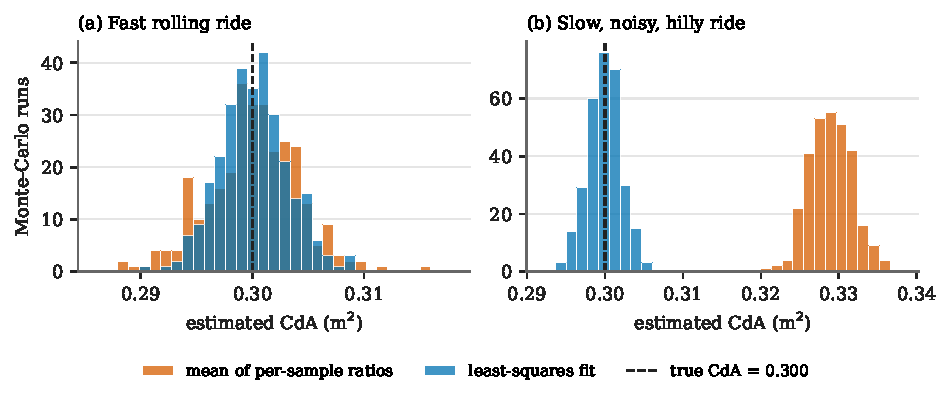
\includegraphics[width=\textwidth]{figs/fig_cda_mc.pdf}
\caption{Distribution of the estimated \(\CdA\) over 300 Monte-Carlo repetitions for two synthetic rides with true \(\CdA=\SI{0.300}{m^2}\). (a)~Fast ride: both estimators are unbiased, the least-squares fit has 25\% lower spread. (b)~Slow, noisy ride: the mean of per-sample ratios is biased by \(+0.029\ \si{m^2}\) (\(+10\%\)) because implausible negative ratios are discarded; the least-squares estimate remains unbiased.}\label{fig:mc}
\end{figure}

\begin{table}[H]
\centering\small
\begin{tabular}{@{}lrrrr@{}}
\toprule
 & \multicolumn{2}{c}{Ride (a)} & \multicolumn{2}{c}{Ride (b)} \\
\cmidrule(lr){2-3}\cmidrule(lr){4-5}
Estimator & mean & s.d. & mean & s.d. \\
\midrule
Least squares, Eq.~\eqref{eq:ls} & 0.3001 & 0.0030 & 0.2999 & 0.0021 \\
Mean of per-sample ratios & 0.3001 & 0.0040 & 0.3290 & 0.0027 \\
\bottomrule
\end{tabular}
\caption{Estimated \(\CdA\) (\si{m^2}); true value 0.300. In the noise-free case the least-squares estimate is 0.3003.}\label{tab:mc}
\end{table}

For ride (a), Eq.~\eqref{eq:varls} predicts that white power noise of \SI{8}{W} alone would give a standard deviation of only \(8/\sqrt{\sum k_i^2}=1.6\times10^{-4}\ \si{m^2}\) (\(\sum k^2=2.5\times10^{9}\)). The observed spread of \(0.003\ \si{m^2}\) --- twenty times larger --- therefore comes almost entirely from the \emph{correlated} errors (grade and speed), which do not average out. This is the central quantitative result for \(\CdA\): \emph{random power noise is irrelevant; systematic errors dominate}.

\subsection{Systematic errors}
\label{sec:sens}
Using the same noise-free ride (a), we perturbed one input at a time and recorded the shift of the fitted value (Table~\ref{tab:sens}, Figure~\ref{fig:sys}).

\begin{figure}[H]
\centering
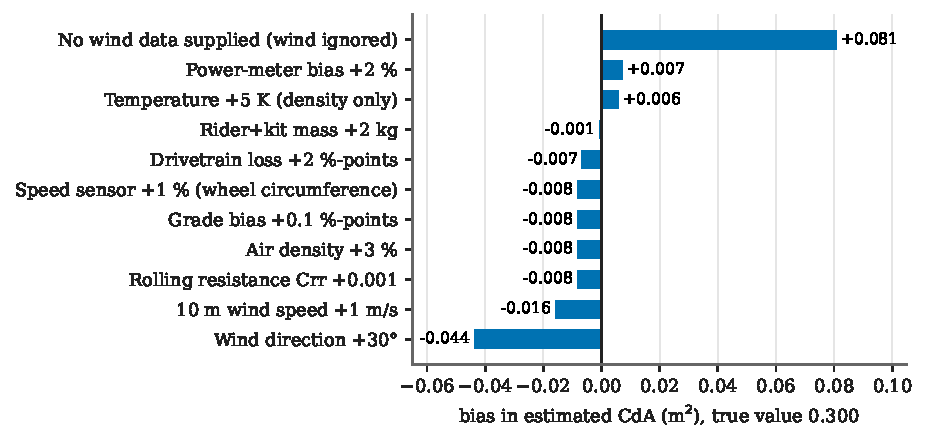
\includegraphics[width=0.92\textwidth]{figs/fig_cda_sys.pdf}
\caption{Bias in the fitted \(\CdA\) caused by single systematic input errors (noise-free ride (a), true value \SI{0.300}{m^2}).}\label{fig:sys}
\end{figure}

\begin{table}[H]
\centering\small
\begin{tabular}{@{}lrr@{}}
\toprule
Perturbation & \(\delta\widehat{\CdA}\) (\si{m^2}) & relative \\
\midrule
No wind data supplied (wind ignored)         & \(+0.081\) & \(+27\%\) \\
Power-meter gain \(+2\%\)                    & \(+0.007\) & \(+2.4\%\) \\
Temperature \(+5\,\si{K}\) (density only)    & \(+0.006\) & \(+2.0\%\) \\
Mass \(+\SI{2}{kg}\)                         & \(-0.001\) & \(-0.3\%\) \\
Drivetrain loss \(+2\) percentage points     & \(-0.007\) & \(-2.3\%\) \\
Speed sensor \(+1\%\)                        & \(-0.008\) & \(-2.8\%\) \\
Grade bias \(+0.1\) percentage points        & \(-0.008\) & \(-2.8\%\) \\
Air density \(+3\%\)                         & \(-0.008\) & \(-2.8\%\) \\
\(C_{rr}\ +0.001\)                           & \(-0.008\) & \(-2.8\%\) \\
10 m wind speed \(+\SI{1}{m/s}\)             & \(-0.016\) & \(-5.3\%\) \\
Wind direction \(+30^\circ\)                 & \(-0.044\) & \(-14.6\%\) \\
\bottomrule
\end{tabular}
\caption{First-order sensitivity of the fitted \(\CdA\) (true \(0.300\ \si{m^2}\)) to single input errors.}\label{tab:sens}
\end{table}

Four lessons follow.
\begin{enumerate}
 \item \textbf{Wind is the largest error source.} Omitting the wind altogether in a ride with \SI{1.4}{m/s} average head wind at rider height inflates \(\CdA\) by \SI{27}{\percent}; a \(30^\circ\) error in wind direction, easily possible with a modelled hourly value, costs \SI{15}{\percent}. The weather data are modelled at a fixed point and hour, not measured on the route; for point-to-point rides along a single heading these errors do not cancel, whereas for loops the first-order effect partially cancels.
 \item \textbf{Grade, rolling resistance and density produce the same signature} and are mutually degenerate at first order (Eq.~\eqref{eq:bias}). An uncertainty of \(\pm0.001\) in \(C_{rr}\) and \(\pm\SI{0.1}{\percent}\) in mean grade each gives \(\pm0.008\ \si{m^2}\) (\(\pm\SI{2.8}{\percent}\)).
 \item \textbf{The sensor calibration matters at the \SI{2}{\percent} level}: power-meter gain, wheel circumference (speed) and drivetrain efficiency.
 \item \textbf{Constant-speed rides are worst.} For a steady \SI{10}{m/s} ride on flat ground a \(+0.001\) error in \(C_{rr}\) moves \(\CdA\) by \(-0.013\ \si{m^2}\), against \(-0.008\ \si{m^2}\) on the rolling ride, because there is no speed variation to separate rolling from drag.
\end{enumerate}
A plausible total uncertainty, combining errors in \(C_{rr}\), grade, wind (\SI{1}{m/s}, \(15^\circ\)) and calibration in quadrature, is of the order of \(\pm0.03\ \si{m^2}\) (\(\approx10\%\)) for a single ride, and more with poor wind data. This is not negligible against the gain from an aerodynamic position change, so \emph{trends over many rides and comparisons under identical conditions are meaningful, absolute single-ride values should be read with caution}.

\subsection{Braking on steep descents}
\label{sec:braking}
We simulated a ride (physical integration, \SI{3600}{s}, true \(\CdA=\SI{0.300}{m^2}\), power \(250\pm60\) W, grades \(\pm7\%\), no wind, no noise) in which the rider stops pedalling and brakes with a constant \SI{40}{N} on descents steeper than \(5\%\) (865\,s, \SI{24}{\percent} of the ride, mean speed \SI{7.6}{m/s} on those samples, mean unmeasured dissipation \(\approx\SI{300}{W}\) of residual per sample). Without the exclusion the fitted \(\CdA\) is \(0.346\ \si{m^2}\) (\(+0.046\), \(+15\%\)); with it, \(0.304\ \si{m^2}\) (\(+0.004\)). The remaining \(+0.004\ \si{m^2}\) is leakage of the braking transients through the \SI{5}{s} smoothing into neighbouring, unfiltered samples. Even though the steep samples carry only \(7\%\) of the total fit weight here, they dominate the error, because every one of them is biased in the same direction. A unit test (\code{test_braking_on_descents_is_not_booked_as_drag}) enforces this behaviour: slowing the rider on steep descents by \SI{20}{\percent} must not change the estimate.

\section{Limitations of the \(\CdA\) model (not corrected in the code)}
\label{sec:limits-cda}
\begin{itemize}
 \item \textbf{Unmeasured dissipation on moderate descents and in corners.} Steep descents (\(<-5\%\)) are excluded (Section~\ref{sec:descents}), but braking before bends, on moderate gradients or in traffic remains in the data, as do cornering and rubbing losses; each makes \(\hat P_{\mathrm{aero}}\) too large and \emph{biases \(\CdA\) upward}. A speed- or curvature-based filter (excluding samples with strong deceleration at \(P=0\)) would remove more of it.
 \item \textbf{Drafting and group riding} reduce the effective \(\CdA\) by tens of percent \citep{crouch2017}; a ride in a group does not measure the free-air value.
 \item \textbf{Yaw dependence, posture changes, standing and sprinting} are not modelled (Section~\ref{sec:balance}).
 \item \textbf{Elevation noise.} Grade is taken from the smoothed altitude profile; short, steep errors in barometric or GPS altitude translate directly into \(P_{\mathrm{grav}}\) errors with the same signature as \(C_{rr}\) (Eq.~\eqref{eq:bias}).
 \item \textbf{Tail wind stronger than ground speed} is mis-signed, and the weather input is a coarse hourly model value (Section~\ref{sec:balance}).
 \item \textbf{Constant \(C_{rr}\) and \(\lambda\)} are assumed; in reality \(C_{rr}\) varies with surface, tyre pressure and (weakly) speed, and \(\lambda\) with power and cadence.
\end{itemize}

%=====================================================================
\part{Two-node model of core and skin temperature}
%=====================================================================
\section{Model structure}
\label{sec:thermal-structure}
Human thermoregulation has been described by models of widely differing complexity, from the two-node model of \citet{gagge1971} to the multi-segment, multi-layer models of \citet{stolwijk1971} and \citet{fiala1999} (see \citealp{havenith2016} for a review). BikeToolsAnalyzer uses a \emph{two-node} model: a \emph{core} node (organs, muscle, deep tissue; 90\% of the body mass) and a \emph{skin} node (10\%), each with a uniform temperature, \(T_c\) and \(T_s\) (Figure~\ref{fig:scheme}). The nodes exchange heat by conduction and blood flow; the skin exchanges heat with the environment by convection/radiation through the clothing and by evaporation of sweat; the core loses heat by breathing.

\begin{figure}[H]
\centering
\small
\setlength{\unitlength}{1mm}
\begin{picture}(130,38)(0,0)
 \put(2,12){\framebox(30,16){\shortstack{\textbf{Core}\\$C_c,\;T_c$}}}
 \put(62,12){\framebox(30,16){\shortstack{\textbf{Skin}\\$C_s,\;T_s$}}}
 \put(32,20){\vector(1,0){30}}
 \put(34,22){$Q_{cs}=K(T_c-T_s)$}
 \put(17,28){\vector(0,1){8}} \put(19,31){$Q_{res}$}
 \put(17,4){\vector(0,1){8}} \put(19,5){$H=M-W$}
 \put(92,22){\vector(1,0){24}} \put(94,24){$Q_{dry}$}
 \put(92,18){\vector(1,0){24}} \put(94,13){$Q_{evap}$}
 \put(118,19){\shortstack[l]{environment\\$T_a,\ \varphi,\ v_{air}$}}
\end{picture}
\caption{Structure of the two-node model. Heat \(H\) is produced in the core; it flows to the skin (\(Q_{cs}\)), is lost to the air by dry exchange and evaporation, and by respiration from the core.}\label{fig:scheme}
\end{figure}

The governing equations are the energy balances of the two nodes,
\begin{align}
 C_c\,\frac{\dd T_c}{\dd t} &= H - Q_{res} - Q_{cs}, \label{eq:core}\\
 C_s\,\frac{\dd T_s}{\dd t} &= Q_{cs} - Q_{dry} - Q_{evap}, \label{eq:skin}
\end{align}
with heat capacities \(C_c=(1-f_s)\,m\,c_c\) and \(C_s=f_s\,m\,c_s\), skin mass fraction \(f_s=0.1\), \(c_c=\SI{3470}{J/(kg\,K)}\), \(c_s=\SI{3500}{J/(kg\,K)}\) (the value commonly used in the Gagge model is \(\approx\SI{3490}{J/(kg\,K)}\)). Adding Eqs.~\eqref{eq:core}--\eqref{eq:skin} shows that the transfer term \(Q_{cs}\) cancels, so the total stored heat changes by exactly
\begin{equation}
 \frac{\dd (C_cT_c+C_sT_s)}{\dd t}=H-Q_{res}-Q_{dry}-Q_{evap},
 \label{eq:energy}
\end{equation}
a property that the discretisation preserves exactly and that we use as a verification test (Section~\ref{sec:thermal-verif}).

\subsection{Body surface area}
Heat-exchange coefficients are defined per unit surface, so the body surface area \(A\) is estimated from height \(H_{cm}\) (cm) and mass \(W\) (kg) with the \citet{dubois1916} formula,
\begin{equation}
 A = 0.007184\;H_{cm}^{0.725}\,W^{0.425}\quad(\si{m^2}),
\end{equation}
which gives \SI{1.60}{m^2} for \SI{165}{cm}/\SI{55}{kg}, \SI{1.85}{m^2} for \SI{175}{cm}/\SI{70}{kg} and \SI{2.09}{m^2} for \SI{185}{cm}/\SI{85}{kg}. The formula is derived for upright standing adults; the effective exchange area on the bicycle (crouched posture, parts of the body shielded) is smaller, which is not corrected for.

\section{Heat production}
\label{sec:heatprod}
Let \(W\ge0\) be the mechanical (crank) power. The metabolic rate is
\begin{equation}
 M=\max\!\left(\frac{W}{\eta},\ M_0A\right),\qquad H=M-W,
 \label{eq:metab}
\end{equation}
with \(M_0=\SI{58.2}{W/m^2}\) the resting metabolic rate (1~met, \citealp{iso7730}) and \(\eta=0.23\) the \emph{gross} efficiency. Only the fraction \(\eta\) of the metabolic energy leaves the body as mechanical work; the remainder, \(H=W(1/\eta-1)\approx3.35\,W\), is heat. Reported gross efficiencies of trained cyclists lie in roughly the range \(18\)--\(25\%\) depending on power, cadence and fitness \citep{ettema2009}. The \(\max\) ensures the rider produces at least the resting heat when freewheeling (without it, an idle rider cooled indefinitely; this was one of the defects corrected during the audit).

Two simplifications deserve mention: (i) \(\eta\) is a constant, whereas it varies with power and with the oxygen-uptake slow component \citep{ettema2009}; (ii) \(M\) responds instantaneously to power, whereas oxygen uptake lags power by about \(30\)--\SI{60}{s}. Both are minor next to the sensitivity to \(\eta\) itself (Section~\ref{sec:thermal-sens}).

\section{Heat exchange with the environment}
\subsection{Dry exchange through the clothing}
\label{sec:dry}
Sensible heat (convection and radiation combined) flows through the series resistance of the clothing and the air boundary layer:
\begin{equation}
 Q_{dry}=\frac{A\,(T_s-T_a)}{R_{cl}+R_{air}(v_{air})},\qquad R_{air}=\frac{1}{h_a},\quad h_a=\max\bigl(\alpha\,v_{air}^{\,n},\ h_0\bigr),
 \label{eq:dry}
\end{equation}
with \(\alpha=8.5\), \(n=0.84\), \(h_0=\SI{7.8}{W/(m^2K)}\) and \(v_{air}\) the \emph{apparent air speed} \(\sqrt{v_a^2+v_\perp^2}\) of Eq.~\eqref{eq:vair} computed with the smoothed ground speed and the wind at rider height (identical to the wind treatment of the drag model; the thermal model previously computed the wind separately). Clothing insulation is
\begin{equation}
 R_{cl}=0.155\sum_j I_j\quad(\si{m^2\,K/W}),
\end{equation}
where \(I_j\) (in clo; \(1\,\mathrm{clo}=\SI{0.155}{m^2K/W}\), \citealp{gagge1941}) is the nominal insulation of each garment from the catalogue (e.g.\ summer jersey 0.15 clo, long-sleeve jersey 0.25 clo, rain jacket 0.35 clo). Summing garment values is the standard first approximation of ISO~9920 \citep{iso9920}.

\paragraph{Assessment.} The coefficient \(h_a=8.5\,v^{0.84}\) is an empirical combined (convective+radiative) coefficient, not a standard correlation. Figure~\ref{fig:h} compares it with the ASHRAE correlation for a clothed standing person, \(h_c=8.3\,v^{0.6}\) (\(0.2<v<\SI{4}{m/s}\), \citealp{ashrae2017}), to which a linearised radiative coefficient \(h_r\approx\SI{4.7}{W/(m^2K)}\) must be added. The model is lower than the standard value at \(v\lesssim3\,\si{m/s}\) and increasingly higher above it (\SI{33}{W/(m^2K)} against \SI{26.5}{} at \SI{5}{m/s}; \SI{59}{} against \SI{38}{} at \SI{10}{m/s}, Table~\ref{tab:h}). At cycling speeds the standard correlation is outside its validated range (\(\le\SI{4}{m/s}\)), so a stronger dependence is not unreasonable: however, the exponent and prefactor have not been calibrated against measurements for cyclists. The consequence is shown in Section~\ref{sec:thermal-sens}: the model is moderately insensitive to \(\alpha\) at moderate temperatures (\(\pm20\%\) in \(\alpha\) changes the final core temperature by \(\lesssim0.15\,\si{K}\)).

\paragraph{Still-air limit.} A pure power law has a serious shortcoming at low speed: \(h_a\to0\) as \(v_{air}\to0\), whereas radiation and natural convection guarantee a floor of about \(4.7+3.1\approx\SI{7.8}{W/(m^2K)}\) even in still air \citep{ashrae2017}. The unfloored model gave \(h_a=\SI{2.2}{W/(m^2K)}\) at \SI{0.2}{m/s}, which kept riders too warm at stops, on slow climbs and at rest (skin \(\approx2\,\si{K}\) too warm; finding~O1). The coefficient is therefore \(h_a=\max(\alpha v_{air}^{\,n},\,h_0)\) with \(h_0=\SI{7.8}{W/(m^2K)}\); the floor is active only below \(\approx\SI{0.9}{m/s}\) and leaves all riding conditions unchanged.

\begin{figure}[H]
\centering
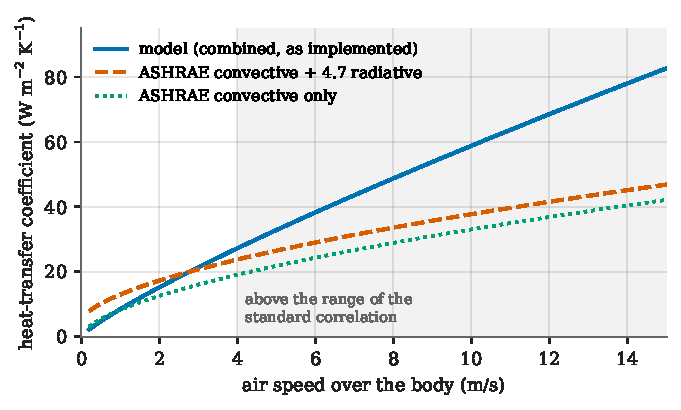
\includegraphics[width=0.62\textwidth]{figs/fig_hconv.pdf}
\caption{Heat-transfer coefficient used by the model compared with the ASHRAE correlation for a clothed person \citep{ashrae2017}.}\label{fig:h}
\end{figure}
\begin{table}[H]
\centering\small
\begin{tabular}{@{}rrrr@{}}
\toprule
\(v_{air}\) (\si{m/s}) & model \(8.5\,v^{0.84}\) & ASHRAE \(8.3\,v^{0.6}\) & ASHRAE \(+\,4.7\) \\
\midrule
1 & 8.5 & 8.3 & 13.0 \\
2 & 15.2 & 12.6 & 17.3 \\
5 & 32.9 & 21.8 & 26.5 \\
10 & 58.8 & 33.0 & 37.7 \\
\bottomrule
\end{tabular}
\caption{Coefficients in \si{W/(m^2K)}.}\label{tab:h}
\end{table}

\paragraph{Clothing under wind.} Insulation measured on a still manikin decreases substantially with wind and movement through air penetration and the pumping effect, by up to about \(40\)--\SI{50}{\percent} in thin ensembles \citep{havenith1990}. The model applies the nominal static value; for a rider moving at \(10\,\si{m/s}\) this overestimates the insulation of non-windproof garments and underestimates it for windproof ones (the catalogue gives a rain jacket \(0.35\) clo regardless of air speed). This is open finding~O6.

\subsection{Evaporative heat loss}
\label{sec:evap}
Evaporation is the dominant heat sink when the body must dissipate heat above what the skin can lose dry. Two quantities limit it: the \emph{sweat supply} \(S\) that the body secretes, and the \emph{evaporative capacity} \(E_{max}\) that the environment allows. In the physical treatment of \citet{gagge1977}, \(E_{max}=h_e\,(p_{s,sk}-p_a)\,A\) with the skin-surface saturation pressure \(p_{s,sk}\) and the ambient vapour pressure \(p_a\), and the evaporative coefficient \(h_e\) related to the convective one by the Lewis relation (\(\approx\SI{16.5}{K/kPa}\)). Our model uses a phenomenological version of this structure:
\begin{align}
 S &= g_s\,\max(0,\,T_c-37),\qquad g_s=\SI{1000}{W/K}, \label{eq:sweat}\\
 E_{max} &= \varepsilon_0\,\max(v_{air},0.2)^{0.3}\,A\,\max\!\left(0,\ \frac{p_{s}(T_s)-\varphi\,p_{s}(T_a)}{p_{s}(\SI{33}{\degreeCelsius})}\right),\qquad \varepsilon_0=\SI{150}{W/m^2},\label{eq:emax}\\
 Q_{evap} &= \min(S,\,E_{max}), \label{eq:qevap}
\end{align}
with \(p_s(T)=\SI{0.6112}{kPa}\,\exp[17.67\,T/(T+243.5)]\) \citep{bolton1980}. The bracket in Eq.~\eqref{eq:emax} is the vapour-pressure gap between wet skin and ambient air, normalised to a skin at \SI{33}{\degreeCelsius} in dry air; it reduces to \(1-\varphi\) when air and skin are at the same temperature, which is the form the model used before the audit. Using \(1-\varphi\) alone, however, made the evaporative capacity independent of temperature, which is wrong: cool humid air (\SI{10}{\degreeCelsius}, \SI{90}{\percent}) has a vapour-pressure gap of \(0.78\) of the dry value for typical skin temperatures, whereas \(1-\varphi\) gives \(0.10\). Eq.~\eqref{eq:emax} corrects this. The \(\max(v_{air},0.2)\) floor prevents the capacity from vanishing in still air (physical body movement and natural convection always provide some air motion).

\paragraph{Assessment.} The sweat supply, Eq.~\eqref{eq:sweat}, has the right order of magnitude --- \(\SI{1000}{W}\) corresponds to about \(\SI{1.5}{L/h}\) of fully evaporated sweat (latent heat \(\approx\SI{2430}{kJ/kg}\)), within the range reported for athletes --- but it is driven only by core temperature, and not, as in Gagge-type controllers, by a weighted combination of core and skin temperatures. \(E_{max}\) is \emph{not} derived from the Lewis relation: at \SI{1}{m/s} and dry air, \(\varepsilon_0=\SI{150}{W/m^2}\) is several times lower than the nude-skin value (\(\approx\SI{16.5}{}\times8.3\times5.03\approx\SI{690}{W/m^2}\)), which is plausible as an effective value for a clothed rider (clothing vapour resistance, sweat dripping rather than evaporating) but is a calibration constant. The speed exponent of \(0.3\) is likewise smaller than the exponent of the convective coefficient. Neither has been fitted to data (open finding~O4).

\subsection{Respiratory heat loss}
The sensible and latent heat lost through breathing is, in the standard formulation of \citet{fanger1970} and \citet{iso7730},
\begin{equation}
 Q_{res}=\max\bigl(0,\ 0.0014\,M\,(34-T_a)+0.0173\,M\,(5.87-p_a)\bigr),
\end{equation}
with \(M\) in W and the ambient vapour pressure \(p_a=\varphi\,p_s(T_a)\) in kPa. The two terms are the dry and the latent loss, both proportional to ventilation, which scales with \(M\). At \SI{200}{W} (\(M=\SI{870}{W}\)) in \SI{20}{\degreeCelsius}, \SI{50}{\percent} RH the formula gives \SI{88}{W}, about \SI{13}{\percent} of the heat produced.

\subsection{Core--skin transfer and vasodilation}
The conductance between core and skin combines tissue conduction with convective transport by skin blood flow:
\begin{equation}
 K = A\left[k_{min}+k_v\,\frac{\sigma}{1+\sigma}\right],\qquad \sigma=\max(0,\,T_c-36.8),
 \label{eq:K}
\end{equation}
\begin{align}
 k_{min}&=\SI{12.6}{W/(m^2K)}=5.28\ (\text{tissue})+7.3\ (\text{skin blood flow}),\\
 k_v&=\SI{150}{W/(m^2K)}.
\end{align}
The basal terms \(5.28\) and \(7.3\) are those of the Gagge model \citep{gagge1971,gagge1977} (minimal skin blood flow of \SI{6.3}{L/(m^2h)}, multiplied by the volumetric heat capacity of blood, \(\SI{1.163}{W\,h/(L\,K)}\)). The saturating vasodilation term is a heuristic: it rises smoothly with the core temperature above \SI{36.8}{\degreeCelsius}, avoids a hard switch, and reaches half its asymptote at \(T_c=37.8\ \si{\degreeCelsius}\). In Gagge-type models skin blood flow increases linearly with the core-temperature error up to a physiological cap of about \SI{90}{L/(m^2h)}, i.e.\ \(\approx\SI{105}{W/(m^2K)}\); the present form reaches that conductance only at \(\sigma\approx1.6\) (\(T_c\approx38.4\) \si{\degreeCelsius}) --- later and more gradually than the physiological controller --- so it is, if anything, \emph{conservative} regarding heat dissipation. It also ignores the inhibition of skin vasodilation by cold skin and the reduction of blood flow to the skin during heavy exercise.

\subsection{Exercise set point}
\label{sec:setpoint}
In exercising humans the steady-state core temperature is not fixed by the environment but rises in proportion to the \emph{relative} workload (fraction of maximal oxygen uptake), almost independently of ambient temperature over a wide range \citep{saltin1966}: the thermoregulatory set point is shifted upward during exercise, so that thresholds for sweating and skin vasodilation are higher than at rest. A model with fixed resting thresholds (\SI{37.0}{\degreeCelsius} and \SI{36.8}{\degreeCelsius}) holds the core at about \SI{37.1}{\degreeCelsius} at \SI{200}{W} in mild air, \(\sim0.8\,\si{K}\) below the measured plateau. We shift both thresholds by
\begin{equation}
 \Delta(t)=g_{sp}\,\phi(t),\qquad
 \frac{\dd\phi}{\dd t}=\frac{\min\!\bigl(W(t)/\mathrm{FTP},\ \phi_{max}\bigr)-\phi}{\tau_{sp}},
 \label{eq:setpoint}
\end{equation}
so that sweat onset is \(37.0+\Delta\) and vasodilation onset \(36.8+\Delta\) (\si{\degreeCelsius}), with \(g_{sp}=\SI{1.0}{K}\) per unit of FTP, \(\phi_{max}=1.2\) and \(\tau_{sp}=\SI{300}{s}\) (the first-order filter reproduces the observed rise of core temperature over the first \(10\)--\SI{20}{min}). The relative intensity is taken as power over the rider's FTP, because the FTP is known to the application while \(\dot V\mathrm{O}_{2,max}\) is not; FTP is a proxy for the lactate threshold, at about \(75\)--\(85\%\) of \(\dot V\mathrm{O}_{2,max}\) in trained riders. Without an FTP the shift is zero and the model reduces to the resting-threshold version. The gain \(g_{sp}\) is chosen to reproduce a core temperature of \(\approx\SI{38}{\degreeCelsius}\) at about \(80\%\) of FTP in mild air; it has \emph{not} been fitted to data, and its effect is shown in Section~\ref{sec:setpoint-results}.

\section{Numerical integration}
\label{sec:numerics}
Equations~\eqref{eq:core}--\eqref{eq:skin} are integrated with the explicit (forward) Euler method with time step \(\Delta t\). For a linear relaxation with time constant \(\tau\), forward Euler is stable only for \(\Delta t<2\tau\), and monotone for \(\Delta t<\tau\) \citep{hairer1993}. The skin node is the stiffest: \(\tau_s=C_s/(K+A/R_{tot})\) ranges from \SI{1050}{s} (resting conductance, no air flow) to \SI{71}{s} (full vasodilation, \SI{10}{m/s} air speed), computed for a \SI{70}{kg}, \SI{175}{cm} rider (\(C_s=\SI{24.5}{kJ/K}\)). The stability limit is therefore \(\Delta t<\SI{141}{s}\). For \SI{1}{Hz} data this holds with a large margin, but \emph{recording gaps and smart-recording files with long intervals could violate it}: we reproduced, with \(\Delta t=\SI{200}{s}\), non-physical skin temperatures of \SI{16}{\degreeCelsius} and jumps of \SI{36}{K} between samples (the original code skipped only intervals above \SI{300}{s}). The integration now subdivides every interval into sub-steps of at most \SI{5}{s}, a factor of \(\approx14\) below the minimum \(\tau_s\). Table~\ref{tab:conv} shows convergence: results are identical for sampling intervals of \(1\) and \SI{5}{s}, and differ by less than \(0.1\ \si{K}\) even for \SI{299}{s}, the residual being due to the sample-and-hold of the inputs rather than to the integrator.

\begin{table}[H]
\centering\small
\begin{tabular}{@{}rrr@{}}
\toprule
Sampling interval (s) & core \(T_c\) at 60 min (\si{\degreeCelsius}) & skin \(T_s\) at 60 min (\si{\degreeCelsius}) \\
\midrule
1 & 39.526 & 36.47 \\
5 & 39.526 & 36.47 \\
60 & 39.508 & 36.45 \\
200 & 39.461 & 36.41 \\
299 & 39.423 & 36.37 \\
\bottomrule
\end{tabular}
\caption{Step-size convergence for \SI{250}{W}, \SI{30}{\degreeCelsius}, \SI{50}{\percent} RH, \SI{8}{m/s}, summer jersey, after the sub-stepping fix. (Before the fix, the \SI{200}{s} and \SI{299}{s} runs diverged.)}\label{tab:conv}
\end{table}

\paragraph{Initial state.} Starting the integration at an arbitrary skin temperature produces a fictitious warm-up transient (the original code used \(T_c=36.0\), \(T_s=\SI{32.0}{\degreeCelsius}\)). The ride now starts with a warm, rested rider, \(T_c=\SI{36.9}{\degreeCelsius}\) (\code{CORE_START_C}), and a skin temperature in quasi-steady balance with the first sample's air and clothing in still air,
\begin{equation}
 T_{s,0}=\frac{k_{min}A\,T_{c,0}+g\,T_a}{k_{min}A+g},\qquad g=\frac{A}{R_{cl}+1/h_0}.
\end{equation}
An earlier version integrated a ``resting equilibrium'' with the same equations; with a realistic still-air coefficient that equilibrium is cold at low ambient temperatures, because the model has no shivering thermogenesis (Section~\ref{sec:limits-thermal}), and so is not a meaningful starting condition.

\section{Verification and behaviour}
\label{sec:thermal-verif}
\subsection{Energy conservation}
Summing Eq.~\eqref{eq:energy} over the simulation shows that the heat stored in the two nodes must equal the integral of generated minus lost heat. This is a pure check on the code, independent of the physics; it holds to the numerical precision of the scheme and is enforced by a unit test (\code{test_energy_is_conserved}).

\subsection{Resting state}
\label{sec:rest}
Table~\ref{tab:rest} shows a rider who sits still after the starting state of Section~\ref{sec:numerics} (no power, no air movement). A resting rider produces \(M_0A=\SI{108}{W}\). At \SI{30}{\degreeCelsius} the core is stable (\(36.9\to37.0\,\si{\degreeCelsius}\)) and skin settles near \SI{35.7}{\degreeCelsius}, as in a warm environment. In cooler air the rider \emph{loses more heat than a resting body produces}: with only a jersey the core falls by \(0.6\,\si{K}\) in an hour at \SI{20}{\degreeCelsius} and by \SI{1.9}{K} at \SI{5}{\degreeCelsius} and \SI{1.4}{K} at \SI{10}{\degreeCelsius} with two layers. Real riders would shiver (raising \(M\) by a factor of 2--3) and vasoconstrict; the model has neither, so \textbf{long stops in cold air are overcooled} (finding~O9). The change from the previous version, in which the resting skin was about \SI{2}{K} too warm and the core was pinned between the controller thresholds, is the consequence of the still-air floor of Section~\ref{sec:dry}.

\begin{table}[H]
\centering\small
\begin{tabular}{@{}rlrrr@{}}
\toprule
\(T_a\) (\si{\degreeCelsius}) & clothing & core, start & core, after 60 min & skin, after 60 min \\
\midrule
5 & jersey + long-sleeve jersey & 36.90 & 35.01 & 26.4 \\
10 & jersey + long-sleeve jersey & 36.90 & 35.54 & 28.2 \\
20 & summer jersey & 36.90 & 36.31 & 30.8 \\
30 & summer jersey & 36.90 & 37.03 & 35.7 \\
\bottomrule
\end{tabular}
\caption{Resting rider (power 0, no air movement), temperatures in \si{\degreeCelsius}.}\label{tab:rest}
\end{table}

\subsection{Exercise scenarios}
Table~\ref{tab:scen} and Figure~\ref{fig:core} show one-hour rides at constant power on flat ground (\SI{8}{m/s}, \SI{50}{\percent} RH, rider \SI{70}{kg}/\SI{175}{cm}, FTP \SI{250}{W}, no wind).

\begin{table}[H]
\centering\small
\begin{tabular}{@{}llrrrr@{}}
\toprule
Power & Conditions & core, 60 min & skin, 60 min & mean \(H\) (W) & mean heat lost (W) \\
\midrule
150 W & \SI{20}{\degreeCelsius}, jersey & 37.55 & 30.3 & 502 & 468 \\
200 W & \SI{10}{\degreeCelsius}, 3 layers & 37.97 & 32.3 & 670 & 586 \\
200 W & \SI{20}{\degreeCelsius}, jersey & 37.90 & 31.3 & 670 & 607 \\
200 W & \SI{30}{\degreeCelsius}, jersey & 38.68 & 35.2 & 670 & 557 \\
300 W & \SI{25}{\degreeCelsius}, jersey & 39.55 & 35.1 & 1004 & 828 \\
\bottomrule
\end{tabular}
\caption{Temperatures in \si{\degreeCelsius}. The ``3 layers'' are summer jersey, long-sleeve jersey and gilet. Mean heat lost is below or close to production because the core is storing heat while the set point rises; the skin cools from its starting value to the exercise value during the first minutes.}\label{tab:scen}
\end{table}

\begin{figure}[H]
\centering
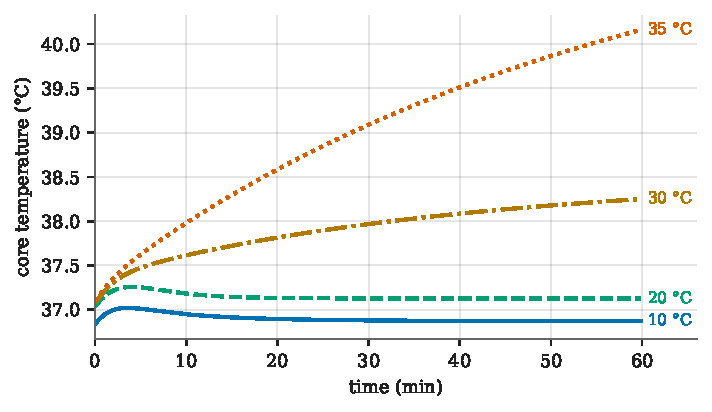
\includegraphics[width=0.62\textwidth]{figs/fig_core_curves.pdf}
\caption{Core temperature during a 60-min ride at \SI{200}{W} (summer jersey, \SI{8}{m/s}, \SI{50}{\percent} RH). In cool and mild air the core temperature rises over the first \(10\)--\SI{20}{min} to a plateau of about \SI{37.7}{}--\SI{37.9}{\degreeCelsius}, as the exercise set point builds up; at \SI{30}{\degreeCelsius} it keeps rising, and at \SI{35}{\degreeCelsius} it reaches \SI{40}{\degreeCelsius}. FTP \SI{250}{W}.}\label{fig:core}
\end{figure}

The qualitative behaviour is that of a thermoregulating body: in cool conditions heat is lost as fast as it is produced (the core stays near \SI{37}{\degreeCelsius}); as the temperature rises, the dry gradient disappears and the core must store heat until sweating (which starts above \SI{37}{\degreeCelsius} plus the exercise set-point shift, Section~\ref{sec:setpoint}) and vasodilation balance production. At \SI{35}{\degreeCelsius} and \SI{60}{\percent} RH the model predicts \(T_c\approx\SI{40.8}{\degreeCelsius}\) after an hour. Experimental studies place exhaustion in hyperthermic exercise at a core temperature of about \SI{40}{\degreeCelsius} \citep{gonzalez1999}; the model has no behavioural feedback (the rider cannot slow down), no dehydration and no cardiovascular limit, so such values should be read as an upper bound on heat storage rather than a forecast.

The effect of humidity is quantified in Figure~\ref{fig:hum}. At \SI{220}{W} and \SI{28}{\degreeCelsius}, increasing relative humidity from 20 to \SI{95}{\percent} raises the one-hour core temperature from \SI{38.3}{} to \SI{39.6}{\degreeCelsius}; at \SI{24}{\degreeCelsius} the same change causes only \(0.3\ \si{K}\), because evaporation is not yet the limiting process. The dependence on RH is monotone in every case, as it must be physically (this is a regression test).

\begin{figure}[H]
\centering
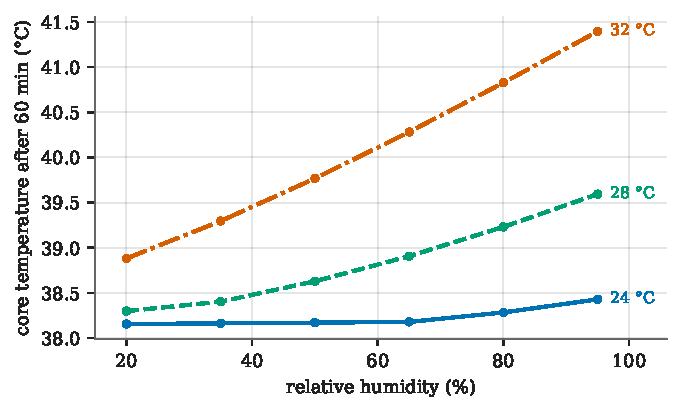
\includegraphics[width=0.62\textwidth]{figs/fig_humidity.pdf}
\caption{Core temperature after \SI{60}{min} at \SI{220}{W} as a function of relative humidity, for three ambient temperatures.}\label{fig:hum}
\end{figure}

\subsection{Effect of the exercise set point}
\label{sec:setpoint-results}
Table~\ref{tab:setpoint} compares one hour at \SI{200}{W} (same conditions as above) without the set-point shift, i.e.\ with the fixed resting thresholds, and with the shift for riders of different FTP. Without it the model predicts about \SI{37.1}{\degreeCelsius} in \SI{20}{\degreeCelsius} air, whereas the measured plateau at a moderately high relative workload is \(\approx38\)--\SI{39}{\degreeCelsius} \citep{saltin1966}; with FTP \SI{250}{W} (\SI{200}{W} \(=80\%\) of FTP) the prediction is \SI{37.9}{\degreeCelsius}. A stronger rider (FTP \SI{400}{W}, \(50\%\)) is less stressed by the same power (\SI{37.6}{\degreeCelsius}), a weaker one (FTP \SI{200}{W}, \(100\%\)) more (\SI{38.1}{\degreeCelsius}), as in the experimental literature. The effect decreases in hot air (\(+0.5\)\,K at \SI{30}{\degreeCelsius} against \(+0.8\)\,K at \SI{20}{\degreeCelsius} for FTP \SI{250}{W}), because the heat-storage regime is then limited by the environment, not by the set point. The gain \(g_{sp}\) is an uncalibrated choice: \(\pm20\%\) of it changes the final core temperature by \(\approx\pm0.13\,\si{K}\) (Figure~\ref{fig:sens}).

\begin{table}[H]
\centering\small
\begin{tabular}{@{}lrrr@{}}
\toprule
 & \SI{10}{\degreeCelsius} (3 layers) & \SI{20}{\degreeCelsius} & \SI{30}{\degreeCelsius} \\
\midrule
Fixed resting thresholds (no FTP) & 36.87 & 37.13 & 38.22 \\
FTP \SI{400}{W} (50\,\%) & 37.36 & 37.61 & 38.49 \\
FTP \SI{250}{W} (80\,\%) & 37.66 & 37.90 & 38.68 \\
FTP \SI{200}{W} (100\,\%) & 37.86 & 38.10 & 38.82 \\
\bottomrule
\end{tabular}
\caption{Core temperature (\si{\degreeCelsius}) after \SI{60}{min} at \SI{200}{W} by rider FTP. The \SI{10}{\degreeCelsius} column uses jersey, long-sleeve jersey and gilet; the others a summer jersey.}\label{tab:setpoint}
\end{table}

\subsection{Parameter sensitivity}
\label{sec:thermal-sens}
Each constant was varied by \(\pm20\%\) (clothing insulation values of all garments scaled together) in two scenarios: a warm one (\SI{220}{W}, \SI{28}{\degreeCelsius}, \SI{50}{\percent}) and a cool one (\SI{180}{W}, \SI{12}{\degreeCelsius}, \SI{70}{\percent}, two layers), both with FTP \SI{250}{W}. Figure~\ref{fig:sens} shows the change in core temperature at 60 minutes.

\begin{figure}[H]
\centering
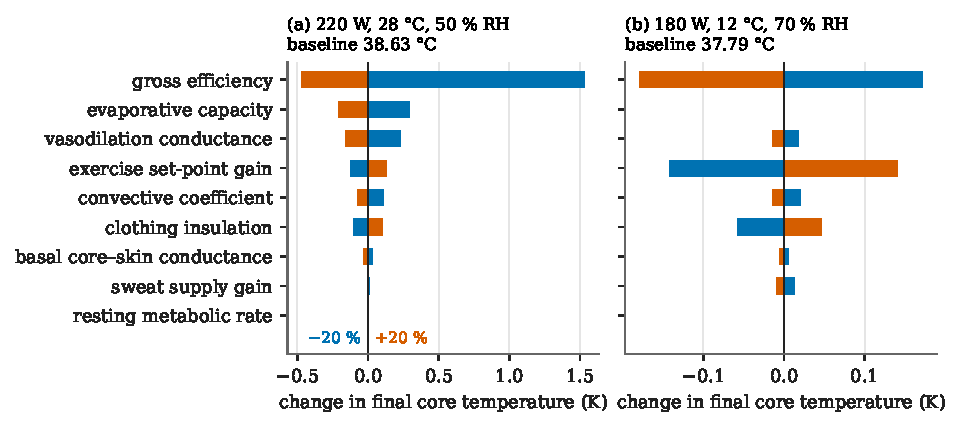
\includegraphics[width=\textwidth]{figs/fig_sens.pdf}
\caption{Sensitivity of the final core temperature to \(\pm20\%\) changes of each model parameter (blue: \(-20\%\); orange: \(+20\%\)). Baselines are \SI{38.63}{\degreeCelsius} (warm) and \SI{37.79}{\degreeCelsius} (cool); FTP \SI{250}{W}.}\label{fig:sens}
\end{figure}

\begin{itemize}
 \item The result in warm conditions is dominated by the \textbf{gross efficiency} \(\eta\): \(\eta=0.184\) (\(-20\%\)) raises the final core temperature by \SI{+1.5}{K} and \(\eta=0.276\) lowers it by \SI{0.5}{K}. The asymmetry arises because the heat produced is \(P(1/\eta-1)\), which changes by \(+32\%\) and \(-22\%\) respectively. Since individual gross efficiency varies at least over \(0.18\)--\(0.25\) \citep{ettema2009}, \emph{the largest uncertainty of the predicted core temperature is the rider's own efficiency}.
 \item The evaporative capacity (\(+0.29/-0.21\,\si{K}\)) and the vasodilation conductance (\(+0.23/-0.16\,\si{K}\)) are next. The set-point gain (\(\pm0.13\,\si{K}\)), the clothing insulation (\(\pm0.10\,\si{K}\)) and the convective coefficient (\(\lesssim0.11\,\si{K}\)) matter less.
 \item In the cool scenario no sweat is secreted and all sensitivities are \(\lesssim0.2\,\si{K}\) (\(\eta\): \(+0.17/-0.18\,\si{K}\); set-point gain \(\pm0.14\,\si{K}\)).
 \item The resting metabolic rate has no effect during exercise, as expected from Eq.~\eqref{eq:metab} (\(W/\eta\gg M_0A\) once \(W>\SI{25}{W}\)).
\end{itemize}

\section{Limitations of the thermal model}
\label{sec:limits-thermal}
\begin{itemize}
 \item \textbf{No calibration or validation against measured core temperature} (e.g.\ with an ingestible pill or a skin-core sensor). The structure and most basal constants come from the literature; the coefficients \(\alpha,n,\varepsilon_0\), the exponent \(0.3\), \(g_s\), \(k_v\), the thresholds and the set-point gain \(g_{sp}\) are heuristic and unvalidated (the gain is chosen to give \(\approx\SI{38}{\degreeCelsius}\) at \(80\%\) of FTP).
 \item \textbf{No cold response.} There is no shivering thermogenesis or cold-induced vasoconstriction: the core of a rider who stops for a long time in cold air falls without limit (Section~\ref{sec:rest}), and skin temperatures in cold air during rides are likely too low.
 \item \textbf{Set point from FTP.} The exercise set point is driven by power over FTP, a proxy for relative intensity; it knows nothing of fitness, fatigue or heat acclimatisation, and reacts to the instantaneous power through a single \SI{300}{s} filter.
 \item \textbf{Solar and radiant load} (direct sun, ground radiation) is not modelled; it is several hundred \si{W} in full sun at midday and shifts the dry heat balance substantially in summer.
 \item \textbf{No state for hydration, acclimatisation, circadian phase or sex differences.} Sweat supply is a single linear function of core temperature.
 \item \textbf{Uniform surface:} one skin temperature, one clothing resistance and one air speed for the whole body; helmet, bare head and hands, and the posture-dependent exposed area are ignored.
 \item \textbf{Clothing:} additive static insulation, without air-layer, fit or wind-penetration effects (Section~\ref{sec:dry}); no moisture accumulation or wetting of the garments.
 \item \textbf{Output semantics:} \code{heat_generated_W} and \code{heat_lost_W} report the values of the \emph{last} sub-step of each sample (relevant only for sampling intervals above \SI{5}{s}).
\end{itemize}

%=====================================================================
\part{Audit summary}
%=====================================================================
\section{Findings register}
Table~\ref{tab:findings} lists the issues found during the audit of both models. ``Fixed'' means corrected in the code together with a regression test (power balance: pull request~\#25; thermal model: pull request~\#26 and the follow-up described in this report).

{\footnotesize\renewcommand{\arraystretch}{1.15}
\begin{longtable}{@{}l>{\raggedright\arraybackslash}p{6.3cm}>{\raggedright\arraybackslash}p{4.6cm}>{\raggedright\arraybackslash}p{2.4cm}@{}}
\caption{Findings register. A = power balance/\(\CdA\); T = thermal, fixed; O = limitations found; the status column says whether they have since been fixed.}\label{tab:findings}\\
\toprule
ID & Finding & Consequence & Status \\
\midrule
\endfirsthead
\toprule
ID & Finding & Consequence & Status \\
\midrule
\endhead
\bottomrule
\endfoot
A1 & Drag-power form \(\tfrac12\rho\CdA v_a^2 v\) and the wind-direction convention (direction the wind blows \emph{from}) corrected and tested & systematic \(\CdA\) error with wind & Fixed \\
A2 & Mean of per-sample ratios, clipped to a window, used as ride \(\CdA\) & upward bias up to \(+10\%\) in noisy rides & Fixed (least squares) \\
A3 & Air density: ISA exponent and humidity (Magnus) & few-percent error in \(\rho\) & Fixed \\
A4 & Tail wind stronger than ground speed has the wrong sign (\(v_a^2\) vs.\ \(v_a|v_a|\)) & rare; wrong \(P_{aero}\) sign in gales & Open \\
A5 & Braking on steep descents booked as drag; fit weights (\(\propto v^6\)) concentrate on fast descents & upward bias (\(+15\%\) in the test ride) & Fixed (descents \(<-5\%\) excluded) \\
A8 & Braking on moderate grades, in bends and in traffic remains in the data & small upward bias & Open \\
A6 & Constant \(C_{rr}\), \(\lambda\), bike mass; \(C_{rr}\) not fitted & aliased into \(\CdA\) (\(\pm0.008\ \si{m^2}\) per \(0.001\)) & Documented \\
A7 & Yaw dependence of \(\CdA\) and drafting ignored & effective, not free-air, \(\CdA\) & Documented \\
\midrule
T1 & No resting heat production (\(M=W/\eta\) only); idle rider cooled to \(\approx\)35.5 \si{\degreeCelsius} & wrong during descents/stops & Fixed \\
T2 & Core--skin conductance omitted basal blood flow (5.28 instead of 12.6 W/m\(^2\)K) & core--skin heat transfer too low & Fixed \\
T3 & Evaporative driving force \(1-\varphi\) instead of the vapour-pressure gap & cool humid air wrongly blocked evaporation & Fixed \\
T4 & Evaporative capacity \(\propto v^{0.3}=0\) in still air & no evaporation at rest/stops & Fixed (floor 0.2 m/s) \\
T5 & Hard-coded initial state 36.0/32.0 \si{\degreeCelsius} & fictitious warm-up transient & Fixed (rest state) \\
T6 & Wind computed separately from, and not consistently with, the drag model (now shared through \code{apparent_air_speed}) & inconsistent air speed between models & Fixed \\
T7 & Forward Euler unstable for sampling intervals \(\gtrsim140\) s & non-physical output for sparse files & Fixed (\(\le5\) s sub-steps) \\
\midrule
O1 & \(h_a\propto v^{0.84}\to0\) at low speed; no still-air floor & skin 2 K warm at rest; slow riding & Fixed (\(h_0=7.8\)) \\
O2 & No exercise-induced set-point shift & core \(\approx0.8\) K too low in mild conditions & Fixed (FTP-driven shift, gain uncalibrated) \\
O3 & Fixed gross efficiency \(\eta=0.23\) & \(\pm1.8/-0.8\) K at \(\pm20\%\) in heat & Documented \\
O4 & Evaporative capacity not from the Lewis relation; clothing vapour resistance and dripping lumped & uncalibrated & Open \\
O5 & No solar or radiant load & underestimates summer heat storage & Open \\
O6 & Clothing insulation static and additive; no wind penetration & over-/underestimate by up to \(\sim\)40\% & Open \\
O7 & Convection exponent/prefactor uncalibrated (higher than ASHRAE above 3 m/s) & overestimates cooling at speed & Open \\
O9 & No shivering or cold vasoconstriction & long stops in cold air overcool; core \(-1.9\) K in 1 h at 5 \si{\degreeCelsius} & Open \\
O8 & Two Magnus parameter sets (Alduchov--Eskridge in density; Bolton in thermal) & \(\approx0.2\%\) difference in \(e_s\); negligible & Documented \\
\end{longtable}}

\section{Recommendations}
\begin{enumerate}
 \item \textbf{Calibrate before trusting absolute values.} Collect a small number of rides with a core-temperature sensor and fit \(\eta\) (or a per-rider efficiency), \(\varepsilon_0\), \(k_v\) and the thresholds; this is the single most valuable step for the thermal model.
 \item \textbf{Fit the set-point gain} \(g_{sp}\) and time constant \(\tau_{sp}\) of Eq.~\eqref{eq:setpoint} together with \(\eta\), and move the exponent/prefactor of the convective coefficient towards the standard \(8.3\,v^{0.6}+4.7\) unless rides show otherwise.
 \item \textbf{Add a minimal cold response} (shivering thermogenesis and cold vasoconstriction) so that long stops in cold air are not overcooled.
 \item \textbf{For \(\CdA\): fit \(C_{rr}\) and \(\CdA\) jointly} on rides with speed variation (regression/virtual-elevation approach, \citealp{martin1998,chung}), also exclude samples with strong deceleration at zero power (bends, braking on moderate grades), and report an uncertainty interval from Table~\ref{tab:sens} alongside the point estimate.
 \item \textbf{Use measured on-route wind where available} (an anemometer or a nearby station), since the modelled wind dominates the uncertainty of single-ride \(\CdA\).
\end{enumerate}

\appendix
\section{Parameters of the thermal model}
\begin{table}[H]
\centering\footnotesize
\begin{tabularx}{\textwidth}{@{}l l l >{\raggedright\arraybackslash}X@{}}
\toprule
Constant & Value & Code & Provenance \\
\midrule
\(c_c\) (core) & \SI{3470}{J/(kg\,K)} & \code{C_BODY} & tissue specific heat; \(\approx\) Gagge \SI{3490}{} \\
\(c_s\) (skin) & \SI{3500}{J/(kg\,K)} & \code{C_SKIN} & as above \\
\(f_s\) skin mass fraction & 0.10 & \code{SKIN_MASS_FRACTION} & Gagge two-node \citep{gagge1971} \\
\(\eta\) gross efficiency & 0.23 & \code{EFFICIENCY} & literature range 0.18--0.25 \citep{ettema2009} \\
\(M_0\) resting metabolism & \SI{58.2}{W/m^2} & \code{M_REST_W_PER_M2} & 1 met, ISO 7730 \\
\(k_{min}\) & \SI{12.6}{W/(m^2K)} & \code{K_MIN_W_PER_M2K} & Gagge: 5.28 + 7.3 \\
\(k_v\) & \SI{150}{W/(m^2K)} & \code{K_VASO_MAX_W_PER_M2K} & \emph{heuristic} \\
vasodilation onset & \SI{36.8}{\degreeCelsius} & \code{VASO_ONSET_CORE_C} & \emph{heuristic} \\
sweat onset & \SI{37.0}{\degreeCelsius} & \code{SWEAT_ONSET_CORE_C} & \emph{heuristic} \\
\(g_s\) sweat gain & \SI{1000}{W/K} & \code{SWEAT_GAIN_W_PER_K} & order of magnitude (\(\approx1.5\) L/h at 1.5 K) \\
\(\varepsilon_0\) evaporative capacity & \SI{150}{W/m^2} & \code{EVAP_COEFF_W_PER_M2} & \emph{calibration}, not Lewis \\
evaporation exponent & 0.3 & \code{EVAP_EXP} & \emph{heuristic} \\
reference skin temperature & \SI{33}{\degreeCelsius} & \code{SWEAT_REF_SKIN_C} & normalisation \\
minimum air speed & \SI{0.2}{m/s} & \code{MIN_AIR_SPEED_MS} & natural convection \\
\(\alpha,\ n\) & 8.5, 0.84 & \code{H_CONV_COEFF, H_CONV_EXP} & \emph{empirical}, see Section~\ref{sec:dry} \\
\(h_0\) still-air floor & \SI{7.8}{W/(m^2K)} & \code{H_STILL_AIR_W_PER_M2K} & radiation 4.7 + natural convection 3.1 \citep{ashrae2017} \\
Start core temperature & \SI{36.9}{\degreeCelsius} & \code{CORE_START_C} & warm, rested rider \\
\(g_{sp}\) set-point gain & \SI{1.0}{K} per FTP & \code{SETPOINT_GAIN_K} & \emph{calibration} to \(\approx38\) \si{\degreeCelsius} at 80\,\% FTP \citep{saltin1966} \\
\(\phi_{max}\) & 1.2 & \code{SETPOINT_MAX_FTP_FRACTION} & \emph{heuristic} \\
\(\tau_{sp}\) & \SI{300}{s} & \code{SETPOINT_TAU_S} & \emph{heuristic} \\
clothing & \(0.155\) m\(^2\)K/W per clo & (inline) & \citep{gagge1941,iso9920} \\
max.\ sub-step & \SI{5}{s} & \code{MAX_SUBSTEP_S} & stability, Section~\ref{sec:numerics} \\
\bottomrule
\end{tabularx}
\caption{Constants of the thermal model.}\label{tab:params-th}
\end{table}

\section{Reproducibility}
\label{app:repro}
The report, its figures and all numerical results are generated by the scripts \code{experiments.py} (Monte Carlo, sensitivity and thermal scenarios), \code{mc_hard.py} (ride (b)) and \code{figs.py} (figures) archived in \code{docs/physics_report/} of the repository; random numbers use fixed seeds. The unit tests in \code{tests/test_aerodyn.py} and \code{tests/test_thermal.py} encode the properties verified here (exclusion of steep descents, apparent wind at rider height, cross wind, head vs.\ tail wind, still-air floor, start state, exercise set point, humidity monotonicity, evaporation in cool humid air, energy conservation and stability for sparse sampling).

\bibliographystyle{plainnat}
\bibliography{refs}
\end{document}
